\documentclass[10pt,letterpaper]{article}

\usepackage[margin=0.75in]{geometry}
\usepackage{tikz}
\usepackage{graphicx}
\usepackage{amsmath}
\graphicspath{{img/}}
\begin{document}

  \title{Stats 314, Data Analysis \#4}
  \author{Cody Malick\\
  \texttt{malickc@oregonstate.edu}}
  \date{\today}
  \maketitle

\section*{Part I}
\subsection*{a}
A total of 256 students were sampled. While 45 were female, 211 were male. 
Based off this data from the graph, there is evidence that less than 25\% of
students identify as female. 

\subsection*{b}
$p=.25$\\
$p<.25$\\

\subsection*{c}
I think that it is an accurate measure as it is an engineers only class. For
that reason, we could take it as a sample of the engineer population. 

\subsection*{d}
It is NOT a random sample.\\
$n*\hat{p} \geq 10$ and $n*(1-\hat{p}) \ge 10$\\
$256*.1757 = 44.979$\\
$256*(1-.1757) = 211.0208$\\ 

It is of sufficient size.

\subsection*{e}
The test statistic uses the following formula:\\\\
$z stat=\frac{\hat{p}-p_0}{\sqrt{\frac{p_0(1-p_0)}{n}}}$\\\\
Plugging in the appropriate values:\\\\
$z stat=\frac{.1757-.25}{\sqrt{\frac{.25(1-.25)}{256}}}=-2.7454$\\

\subsection*{f}
Lower one sided p-stat, equal to $.003022$

\subsection*{g}
The confidence interval formula for a one proportion z test is:\\
$\hat{p} \pm z^* \sqrt{\frac{\hat{p}(1-\hat{p})}{n}}$\\\\
$.1757 \pm 1.96 * \sqrt{\frac{.1757(1-.1757)}{256}}$\\\\
$=.2223$ and $.1291$\\\\

95\% CI from .1291 to .2223

\subsection*{h}
There is moderate evidence that the proportion of students who identify as
female is less than .25. The sample estimates the average proportion of females
to be .1767, with a 95\% confidence interval from .1291 to .2223. The null
hypothesis is rejected at significance value .05. The university should receive
funding to actively market to women to get an engineering or computer science
degree.

\section*{Part II}
\subsection*{a}
The parameter of interest is the proportion of "guzzlers" models in American
and international car companies. 
\subsection*{b}
$p=0$\\
$p \neq 0$\\
\subsection*{c}
Conditions:\\
Random Sample: No, the EPA site says: "The test data used to determine fuel
economy estimates is derived from vehicle testing done at EPA's National Vehicle
and Fuel Emissions Laboratory in Ann Arbor, Michigan, and by vehicle
manufacturers who submit their own test data to EPA.\\
Manufactures submit their own voluntary data. 

Number of successes and failures in each group must be greater than 10:
From our data set, only 7 of the 267 vehicles from America are considered
guzzlers. This does not pass the required level. International does meet the
requirement with 48 success, and plenty more failure.

\subsection*{d}
Test statistic:\\
$z stat=\frac{\hat{p_1}-\hat{p_2}-0}
{\sqrt{\hat{p}(1-\hat{p}(\frac{1}{n_1}+\frac{1}{n_2})}}$\\\\

$\hat{p}=\frac{7+48}{267+581}=\frac{55}{848}=.064858$\\\\
$\hat{p_1}=\frac{7}{267}=.0262$\\\\
$\hat{p_2}=\frac{48}{581}=.0826$\\\\

$z stat=\frac{.0262-.0826}
{\sqrt{.06485(1-.06485)(\frac{1}{267}+\frac{1}{581})}}=-3.0976$\\\\

\subsection*{e}
$p-value=0.000975$

\subsection*{f}
$CI=(\hat{p_1}-\hat{p_2}) \pm z^* \sqrt{\frac{\hat{p_1}(1-\hat{p_1})}{n_1}+
\frac{\hat{p_2}(1-\hat{p_2})}{n_2}}$\\\\
$CI=(.0262-.0826) \pm 1.645 * \sqrt{\frac{.0262(1-.0262)}{267}+
\frac{.0826(1-.0826)}{581}}$\\\\
$=-.03167$ and $-.08112$\\

90\% CI from -.08112 to -.03167

\subsection*{g}
There is slightly convincing evidence that the proportion of gas guzzling
models in American made cars is different than international models. The 90\%
confidence interval estimates the proportion of American models that are gas
guzzlers is -.08112 to .03167 less than international model cars with a point
estimate of .06485 less. The null hypothesis is rejected at a significance level
of .10 (Z=-3.0976, two-sided p-value = .000975).

\section*{Part III}
\subsection*{a}
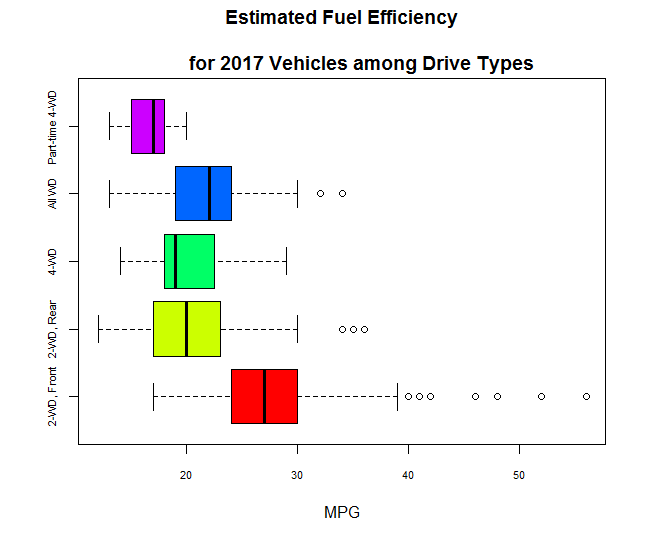
\includegraphics[scale=1.0]{anova}\\
There does seem to be a difference in the average combined fuel efficiency. We
can see by the different inter-quartile ranges that the average does vary from
drive type to drive type.

\subsection*{b}
$H_0:\mu_1 = \mu_2 = \mu_3 = \mu_4 = \mu_5$\\\\
$H_\alpha:$at least two $\mu_is$ differ

\subsection*{c}
Conditions:\\
Samples are obtained using random mechanism: As stated in part II, they are not
random samples.\\
Populations are independent: Populations are independent\\
Populations are normal: Based off the visual data, the distributions are not all
normally distributed.\\
Population standard deviations are the same: Not all the standard deviations are
the same.\\

\subsection*{d}
\subsubsection*{a}
\begin{center}
         \begin{tabular}{l | c | c | c | c | c | r}
		 - & Df & Sum Sq & F value & Pr(>F) &  &  \\
		 fueldata\$Drive & 4 & 9221 & 2305 & 115.4 & 2e-16 *** \\
		 Residuals & 843 & 16845  & 20 &  &  &  \\ 
         \end{tabular}
\end{center}
Signif. codes:  0 *** 0.001 ** 0.01 * 0.05 . 0.1   1

\subsubsection*{b}
The significance value is rejected at .05, as the f-value is very low, close
to zero.

\subsubsection*{c}
The evidence to reject is moderate at a .05 significance value.

\subsection*{e}
\subsubsection*{a}
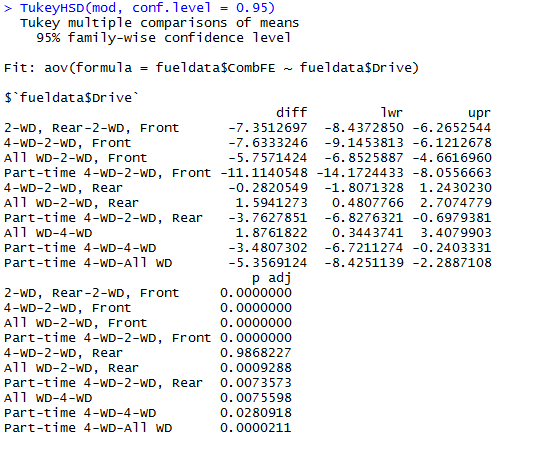
\includegraphics[scale=1.0]{turkey}\\
\subsubsection*{b}
Part-time 4-WD-2-WD, Front -11.1140548 -14.1724433 -8.0556663\\
2-WD, Rear-2-WD, Front      -7.3512697  -8.4372850 -6.2652544\\
4-WD-2-WD, Front            -7.6333246  -9.1453813 -6.1212678\\
Part-time 4-WD-All WD       -5.3569124  -8.4251139 -2.2887108\\

Part-time 4-WD-2-WD has the largest difference in MPG. 8.055 MPG difference.
\subsection*{f}
Two Seaters                 Minicompact Cars\\
Minicompact Cars            Standard SUV 4WD  \\         
Standard SUV 4WD            Standard SUV 4WD    \\      
Standard SUV 4WD            Standard Pick-up Trucks 4WD\\
Standard Pick-up Trucks 4WD Small Pick-up Trucks 4WD   \\
Small Pick-up Trucks 4WD    Small Pick-up Trucks 4WD   \\
Small Pick-up Trucks 4WD    Small Pick-up Trucks 4WD   \\
Standard Pick-up Trucks 4WD Standard Pick-up Trucks 4WD\\
Standard Pick-up Trucks 4WD


This make great sense for fuel efficiency as 4-WD tend to have lower MPG. 

\end{document}
